\documentclass[letterpaper]{article}

\usepackage{enumitem}
\usepackage{listings}
\usepackage{color}
\usepackage{float}
\usepackage{graphicx}
\usepackage{amsmath}
\usepackage{hyperref}
\usepackage{tabularx}
\usepackage{cellspace}
\usepackage{booktabs}

\graphicspath{ {./Figures/} }

\definecolor{dkgreen}{rgb}{0,0.6,0}
\definecolor{gray}{rgb}{0.5,0.5,0.5}
\definecolor{mauve}{rgb}{0.58,0,0.82}

\lstset{frame=tb,
  language=Python,
  aboveskip=3mm,
  belowskip=3mm,
  showstringspaces=false,
  columns=flexible,
  basicstyle={\small\ttfamily},
  numbers=none,
  numberstyle=\tiny\color{gray},
  keywordstyle=\color{blue},
  commentstyle=\color{dkgreen},
  stringstyle=\color{mauve},
  breaklines=true,
  breakatwhitespace=true,
  tabsize=3
}

\begin{document}

\section{K-means}

\subsection{Learning K-means}

\subsubsection{Distance Function}
\label{distance_func}

\begin{lstlisting}
def distance_func(X, mu):
    """ Inputs:
          X: is an NxD matrix (N observations and D dimensions)
          mu: is an KxD matrix (K means and D dimensions)
          
        Output:
          pair_dist: is the squared pairwise distance matrix (NxK)
    """
    broad_X = tf.expand_dims(X, axis=1)
    broad_mu = tf.expand_dims(mu, axis=0)

    return tf.reduce_sum(
        tf.square(tf.subtract(broad_X, broad_mu)),
        axis=-1
    )
\end{lstlisting}

\noindent
The subtraction operation can be broadcasted by expanding different dimensions for $X$ and $\mu$. As provided by the hint in the assignment, both variables are expanded as such:

\begin{align*}
X' \in \mathcal{R}^{N \times 1 \times D} \\
\mu' \in \mathcal{R}^{1 \times K \times D}
\end{align*}

\noindent
The \texttt{tf.subtract()} function will then broadcast the subtraction operation across the first and second axes, producing the pairwise differences. These differences are squared and summed across the last axis $D$ to produce a distance tensor $\delta \in \mathcal{R}^{N \times K}$.

\subsubsection{Training without Validation}

\begin{figure}[H]
	\centering
	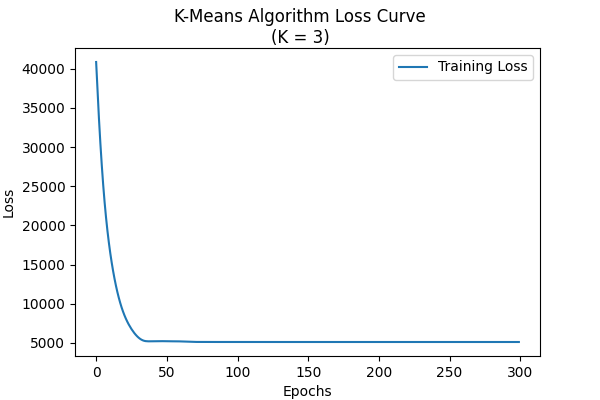
\includegraphics[width=\linewidth]{Figure_1}
	\caption{$K = 3$ with no validation dataset}
	\label{fig:plot1}
\end{figure}

\subsubsection{Training with Validation}

\begin{figure}[H]
	\centering
	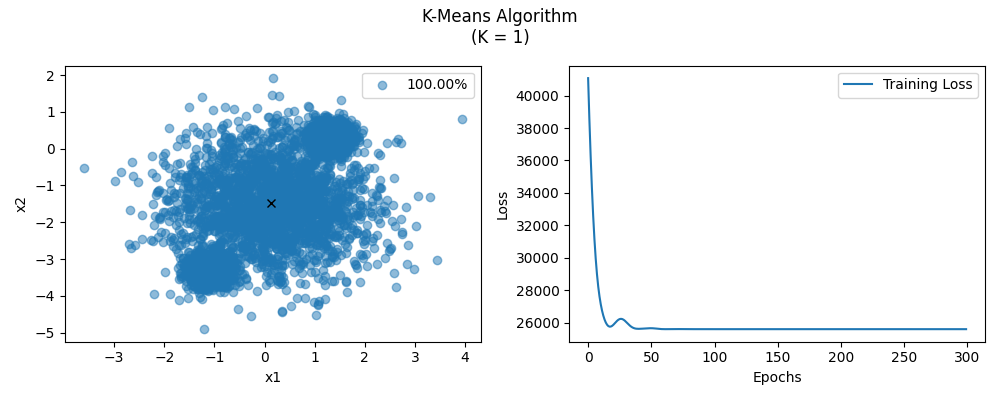
\includegraphics[width=\linewidth]{Figure_2}
	\caption{Validation loss $ = 12870.104$}
	\label{fig:plot2}
\end{figure}

\begin{figure}[H]
	\centering
	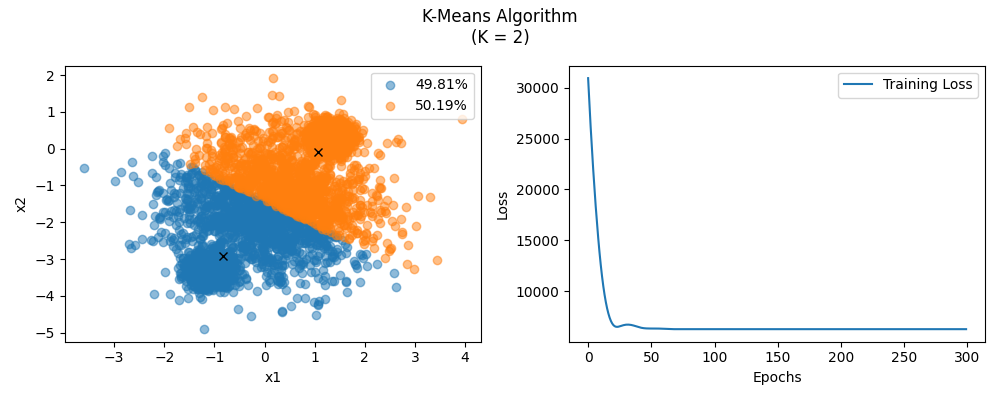
\includegraphics[width=\linewidth]{Figure_3}
	\caption{Validation loss $ = 2960.673$}
	\label{fig:plot3}
\end{figure}

\begin{figure}[H]
	\centering
	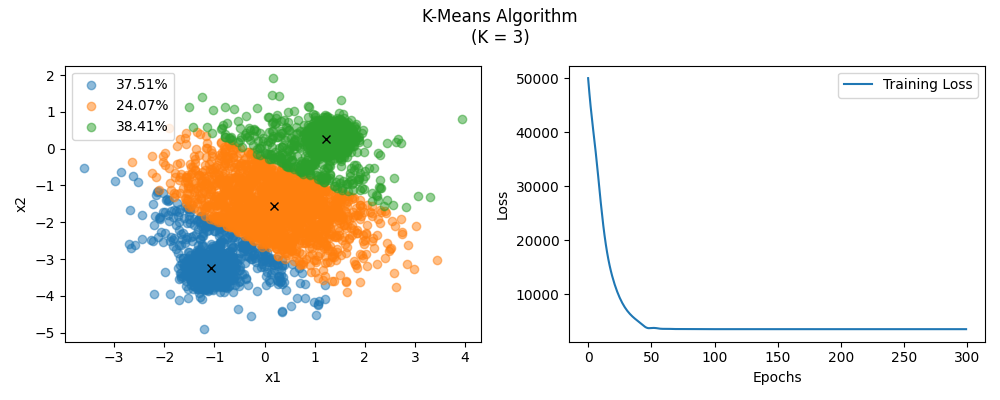
\includegraphics[width=\linewidth]{Figure_4}
	\caption{Validation loss $ = 1629.309$}
	\label{fig:plot4}
\end{figure}

\begin{figure}[H]
	\centering
	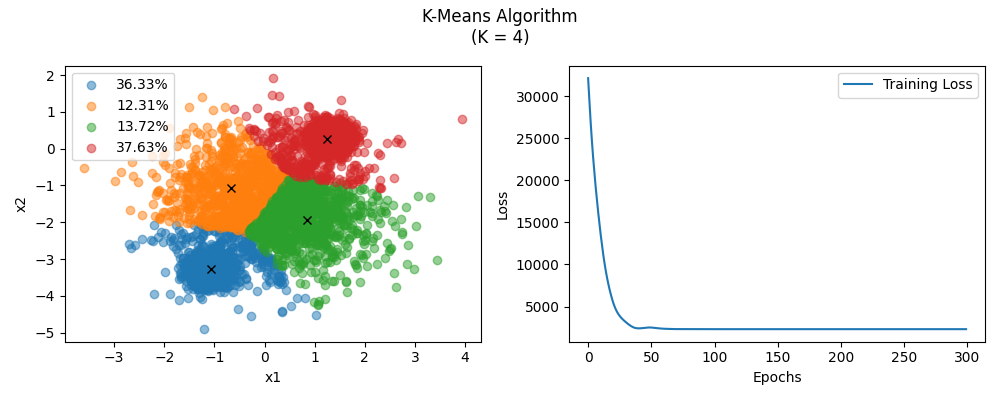
\includegraphics[width=\linewidth]{Figure_5}
	\caption{Validation loss $ = 1054.538$}
	\label{fig:plot5}
\end{figure}

\begin{figure}[H]
	\centering
	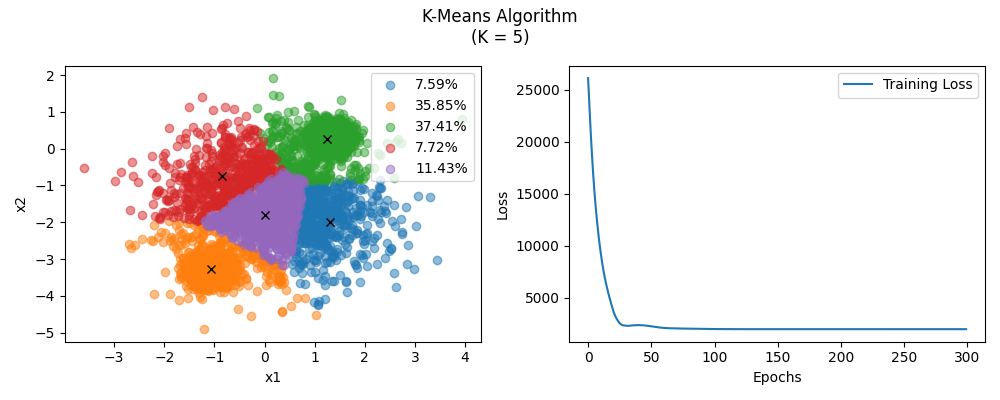
\includegraphics[width=\linewidth]{Figure_6}
	\caption{Validation loss $ = 900.777$}
	\label{fig:plot6}
\end{figure}

\noindent
For a seemingly uniformly-random dataset, as the number of clusters increase, there is a natural tendency for the clusters to maximize the distances between each other, in order to minimize the distances to neighbouring data points. It can be argued that as the number of clusters approach the number of data points, the validation loss will decrease, until it reaches a critical limit of $N = K$, at which point the validation loss will be $0$ and the system is perfect. This behaviour is reflected in the gradually decreasing validation loss from figures \ref{fig:plot2} to \ref{fig:plot6}. From the validation loss alone, the optimal value is $K = 5$, which could be ``optimized'' further by increasing $K$. 

As a result, deciding on a value for $K$ solely based on the minimum loss is misguided. By observing the general spread of data, there are two clear clusters around $(1.5, 0.5)$ and $(-1, -3.5)$, with one large cluster around $(0, -2)$. Without any additional information about the nature of data, the best estimation is $K = 3$.

\newpage

\section{Mixtures of Gaussians}

\subsection{The Gaussian Cluster Mode}

\subsubsection{Log Probability Density Function}
\label{log_gauss_pdf}

\begin{align*}
\log P(\textbf{x} | z = k) &= \log \mathcal{N}(\textbf{x}; \mu_k, \sigma_k^2) \\
&=
\log \left[ \frac{1}{(2 \pi)^{\frac{d}{2}} |\Sigma|^{\frac{1}{2}}} e^{-\frac{1}{2} (x_i - \mu_k)^T \Sigma^{-1} (x_i - \mu_k)} \right] \\
&= 
\log \left[ \frac{1}{(2 \pi)^{\frac{d}{2}} \sigma^d} e^{-\frac{1}{2} \frac{(x_i - \mu_k)^T(x_i - \mu_k)}{\sigma^2}} \right] \\
&=
\log \left[ \frac{1}{\left(\sqrt{2 \pi} \sigma\right)^d} e^{-\frac{1}{2 \sigma^2} (x_i - \mu_k)^2} \right] \\
&= \label{eqn:1} \tag{1}
-d \log \left(\sqrt{2 \pi} \sigma\right) - \left( \frac{1}{2 \sigma^2} (x_i - \mu_k)^2 \right)
\end{align*}

\noindent
In the final simplification shown in equation \ref{eqn:1}, the squared difference $(x_i - \mu_k)^2$ between the observation and the mean of the $k$\textsuperscript{th} cluster is equivalent to the Euclidean distance function for K-means, as shown in section \ref{distance_func}.

\begin{lstlisting}
def log_gauss_pdf(X, mu, sigma):
    """ Inputs: 
            X: N X D
            mu: K X D
            sigma: K X 1

        Outputs:
            log Gaussian PDF (N X K)
    """

    # sigma_T: 1 X K
    sigma_T = tf.transpose(sigma)
    
    distance = starter_kmeans.distance_func(X, mu)
    return tf.subtract(
        tf.multiply(-dim, tf.math.log(tf.sqrt(2 * np.pi) * sigma_T)),
        tf.divide(distance, (2 * tf.square(sigma_T)))
    )
\end{lstlisting}

\noindent
\textit{It is important to note that since $\sigma \in \mathcal{R}^{K \times 1}$, it must be transposed to broadcast operations with \texttt{distance} and produce an output shape of $N \times K$.}

\newpage

\subsubsection{Log Probability}

\begin{align*}
\log P(z | \textbf{x}) &= \log \left[ \frac{P(\textbf{x}, z = k)}{\sum_{j = 1}^{K} P(\textbf{x}, z = j)} \right] \\
&= 
\log \left[ \frac{P(\textbf{x} | z = k) P(z = k)}{\sum_{j = 1}^{K} P(\textbf{x} | z = j) P(z = j)} \right] \\
&=
\log \left[ \frac{P(\textbf{x} | z = k) \pi_k}{\sum_{j = 1}^{K} P(\textbf{x} | z = j) \pi_j} \right] \\
&= \label{eqn:2} \tag{2}
\log P(\textbf{x} | z = k) + \log \pi_k - \log \left[ \sum_{j = 1}^{K} P(\textbf{x} | z = j) \pi_j \right] \\
&= 
\log P(\textbf{x} | z = k) + \log \pi_k - \log \left[ \sum_{j = 1}^{K} e^{\log P(\textbf{x} | z = j) \pi_j} \right] \\
&= \label{eqn:3} \tag{3}
\log P(\textbf{x} | z = k) + \log \pi_k - \log \left[ \sum_{j = 1}^{K} e^{\log P(\textbf{x} | z = j) + \log \pi_j} \right]
\end{align*}

\noindent
Comparing equation \ref{eqn:2} and \ref{eqn:3}, equation \ref{eqn:2} may seem like the better choice as it is simpler. In terms of mathematical computation, however, equation \ref{eqn:3} maximizes the amount of computational overlap for $\log P(\textbf{x} | z = k)$ and $\log \pi_k$ by converting the probability within the summation into its logarithmic form. This allows the reuse of the logarithmic Gaussian probability density function in section \ref{log_gauss_pdf} in conjunction with \texttt{reduce\_sumlogexp()}, which applies a logarithm after the summation of exponents: $\log \sum e^{x}$. Calculating either equation with \texttt{tf.reduce\_sum()} would require the calculation of $P(\textbf{x} | z = j)$ or cost additional work. 

\begin{lstlisting}
def log_posterior(log_PDF, log_pi):
    """ Inputs:
            log_PDF: log Gaussian PDF N X K
            log_pi: K X 1

        Outputs
            log_post: N X K
    """
    
    # Avoid computational redundancy
    sum_log_PDF_pi = tf.add(log_PDF, tf.transpose(log_pi))
    return tf.subtract(
        sum_log_PDF_pi,
        hlp.reduce_logsumexp(sum_log_PDF_pi, keepdims=True)
    )
\end{lstlisting}

\newpage

\subsection{Learning the MoG}

\subsubsection{Negative Log Likelihood}

\begin{align*}
\mathcal{L}(\mu, \sigma, \pi) &= -\log P(\textbf{x}) \\
&=
-\log \left[ \sum_{j = 1}^{K} P(\textbf{x} | z = j) P(z = j) \right] \\
&=
-\log \left[ \sum_{j = 1}^{K} P(\textbf{x} | z = j) \pi_j \right] \\
&=
-\log \left[ \sum_{j = 1}^{K} e^{\log P(\textbf{x} | z = j) \pi_j} \right] \\
&=
-\log \left[ \sum_{j = 1}^{K} e^{\log P(\textbf{x} | z = j) + \log \pi_j} \right] \\
\end{align*}

\subsubsection{Training without Validation}

\begin{figure}[H]
	\centering
	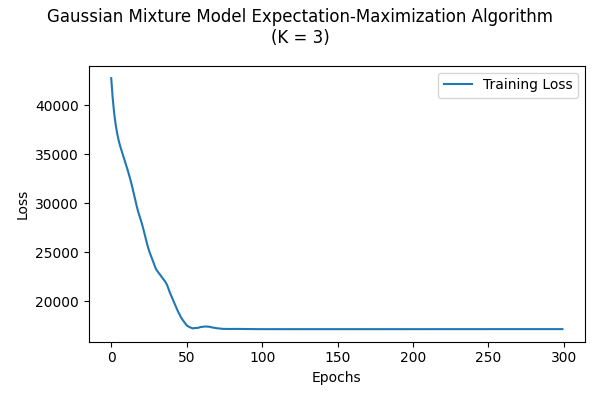
\includegraphics[width=\linewidth]{Figure_7}
	\caption{$K = 3$ with no validation dataset}
	\label{fig:plot7}
\end{figure}

\subsubsection{Training with Validation}

\begin{figure}[H]
	\centering
	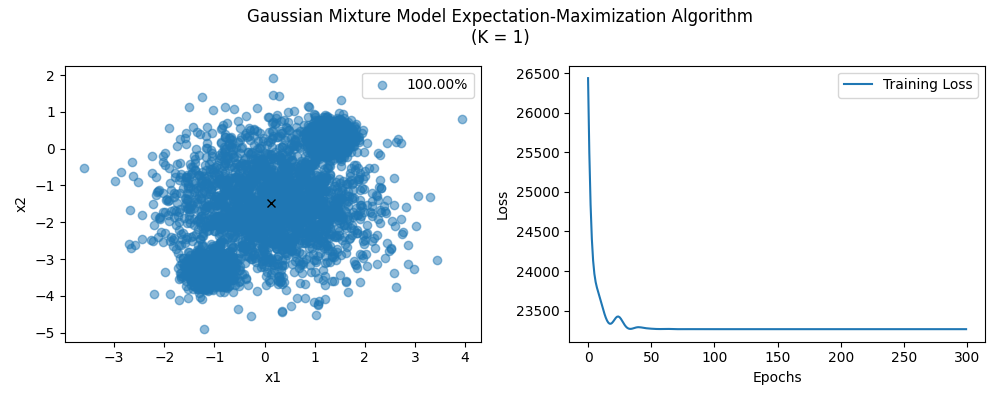
\includegraphics[width=\linewidth]{Figure_8}
	\caption{Validation loss $ = 11651.442$}
	\label{fig:plot8}
\end{figure}

\begin{figure}[H]
	\centering
	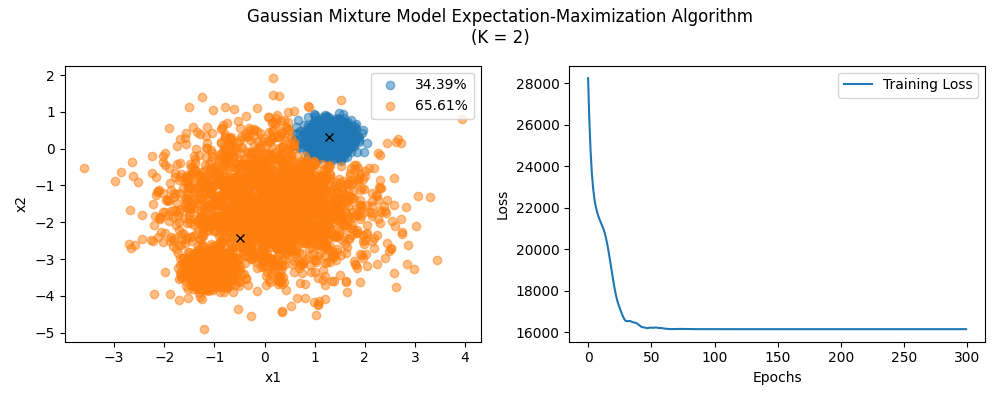
\includegraphics[width=\linewidth]{Figure_9}
	\caption{Validation loss $ = 7987.788$}
	\label{fig:plot9}
\end{figure}

\begin{figure}[H]
	\centering
	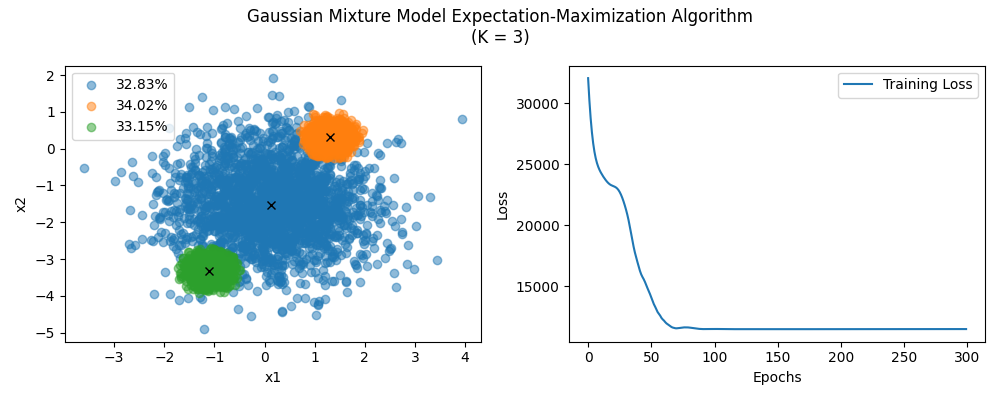
\includegraphics[width=\linewidth]{Figure_10}
	\caption{Validation loss $ = 5635.476$}
	\label{fig:plot10}
\end{figure}

\begin{figure}[H]
	\centering
	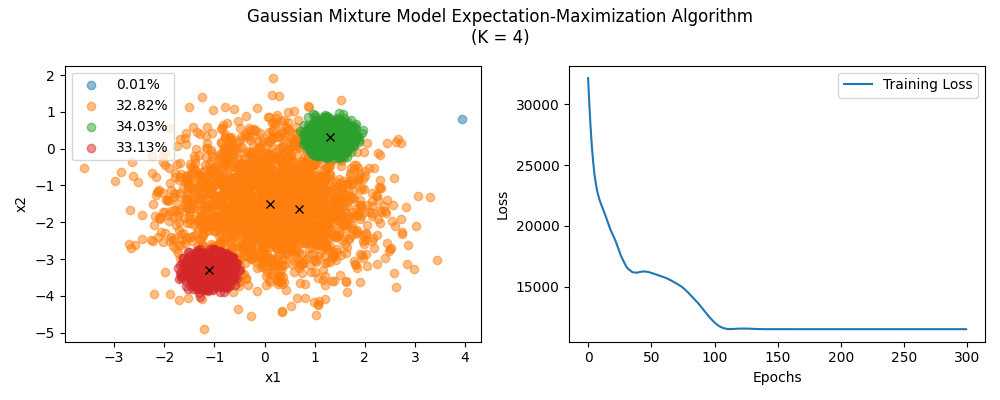
\includegraphics[width=\linewidth]{Figure_11}
	\caption{Validation loss $ = 5630.384$}
	\label{fig:plot11}
\end{figure}

\begin{figure}[H]
	\centering
	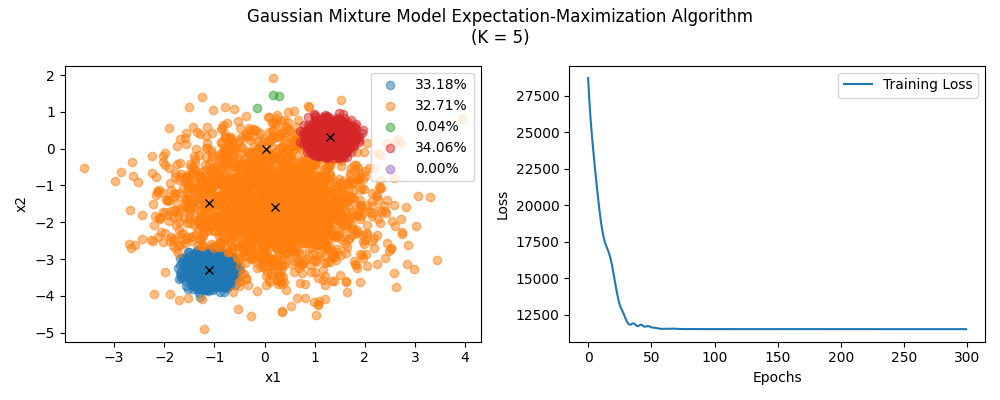
\includegraphics[width=\linewidth]{Figure_12}
	\caption{Validation loss $ = 5630.391$}
	\label{fig:plot12}
\end{figure}

The cluster-loss issue with the K-means algorithm does not apply here. While K-means attempts to utilize every cluster to minimize the total loss, the expectation-maximization algorithm will ``disregard'' some clusters if they do not provide a large enough posterior probability of membership. 

Noticeable from figure \ref{fig:plot10} onwards, as $K \ge 3$, the validation loss has a negligible increase as more clusters are added. The new cluster in figure \ref{fig:plot11} has a $0.04\%$ data point membership, while the fifth cluster in figure \ref{fig:plot12} is completely unused. This indicates that it is most probable that there are a total of $3$ Gaussian clusters in the model, and attempting to include more clusters than $3$ will yield diminishing returns. Figure \ref{fig:plot10} will have the minimum theoretical validation loss, and thus the optimal number of clusters is $K = 3$.

\subsection{\texttt{data100D.npy} Dataset (K-means vs. MoG Learning)}

\subsubsection{K-means}

\begin{tabularx}{\textwidth}{X|XXXXX}
 \toprule
 Cluster & Loss\footnote{Validation loss} & Maximum\footnote{Values for the membership percentage of all clusters} & Median & Minimum \\
 \midrule
 $K = 5$ & $121731.727$ & $30.37\%$ & $20.04\%$ & $10.05\%$ \\
 $K = 10$ & $71230.969$ & $29.29\%$ & $8.74\%$ & $0.00\%$ \\
 $K = 15$ & $69969.008$ & $29.31\%$ & $3.00\%$ & $0.00\%$ \\
 $K = 20$ & $70461.008$ & $20.35\%$ & $0.00\%$ & $0.00\%$ \\
 $K = 30$ & $68927.898$ & $20.35\%$ & $1.31\%$ & $0.00\%$ \\
 \bottomrule
\end{tabularx}

\subsubsection{MoG Learning}

\begin{tabularx}{\textwidth}{X|XXXXX}
 \toprule
 Cluster & Loss & Maximum & Median & Minimum \\
 \midrule
 $K = 5$ & $272222.594$ & $49.66\%$ & $20.04\%$ & $0.00\%$ \\
 $K = 10$ & $163250.906$ & $29.31\%$ & $5.01\%$ & $0.00\%$ \\
 $K = 15$ & $163248.297$ & $29.31\%$ & $0.00\%$ & $0.00\%$ \\
 $K = 20$ & $161845.266$ & $20.35\%$ & $0.00\%$ & $0.00\%$ \\
 $K = 30$ & $162633.234$ & $29.31\%$ & $0.00\%$ & $0.00\%$ \\
 \bottomrule
\end{tabularx}

\subsubsection{Analysis}

For both K-means and MoG learning, the validation loss plateaus and not all clusters are used from $K \ge 10$ onwards. This indicates that the optimal cluster structure can be reached with cluster counts of $K < 10$. Observing the zeroed median value for cluster $K = 15$ for MoG learning, an even tighter bound of $K \le 15 // 2 = 8$ can be inferred. Since no more information can be extracted from the data collected, the estimation for the optimal number of clusters is $5 < K \le 8$, or $K = 7$ to estimate further. Both MoG and K-means seem to reach similar cluster structures, both achieving a maximum membership percentage of $\approx 30\%$ in post-optimal conditions. 

\end{document}
